\section{Client Server}
For this part of the assignment, I chose to use UTF based sockets. The reason
for this, is that they are simple to use and fit the requirement well (we are
only interested in the value and not timestamp, etc.).

\begin{figure}
\caption{Sensor Client}
\centering
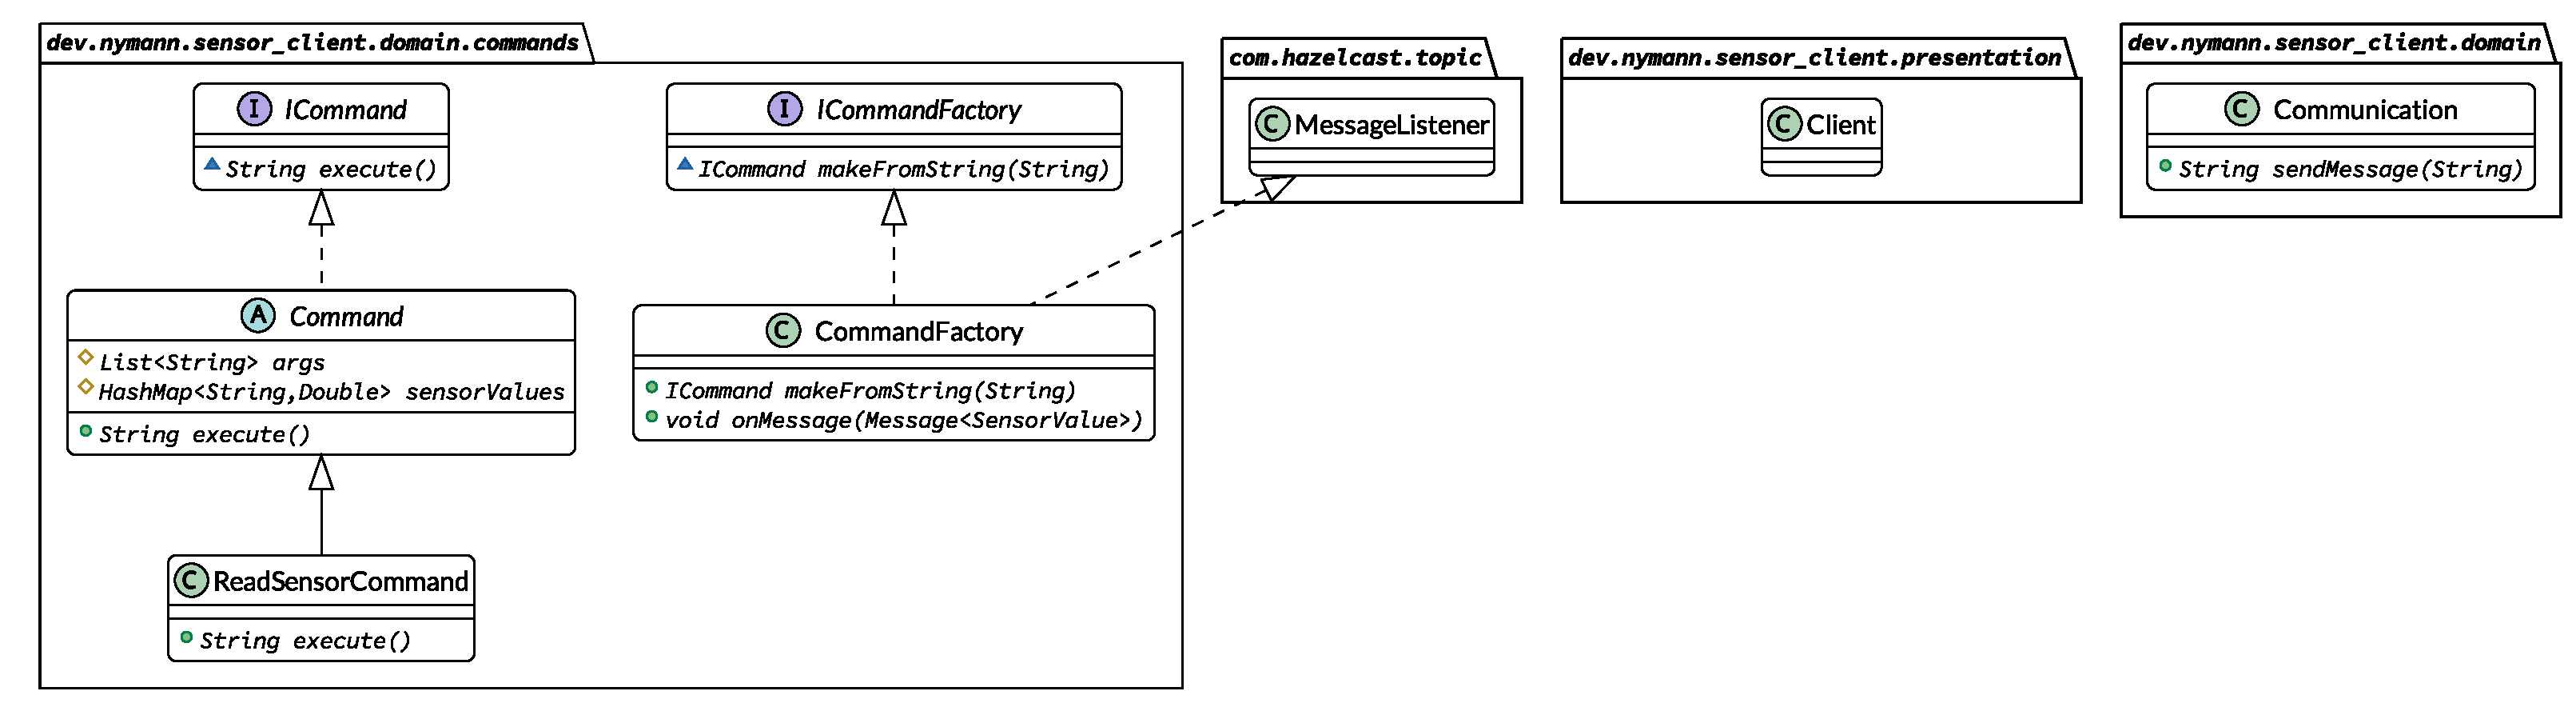
\includegraphics[scale=0.3]{part_two/sensor-client}
\end{figure}

\begin{figure}
\caption{Sensor Server}
\centering
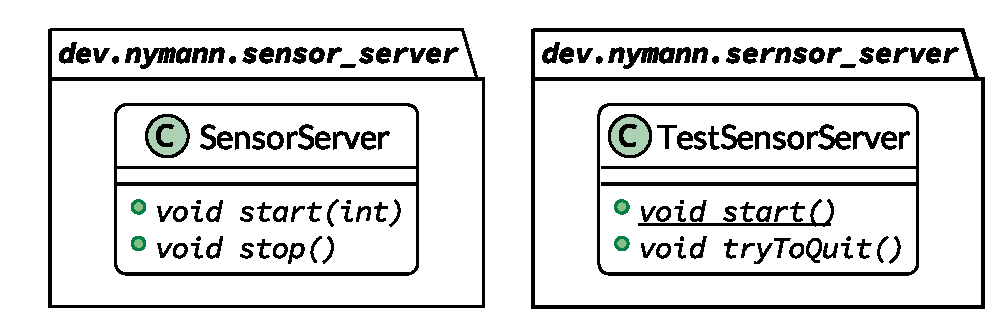
\includegraphics[scale=0.8]{part_two/sensor-server}
\end{figure}

\begin{figure}
\caption{Sensor}
\centering
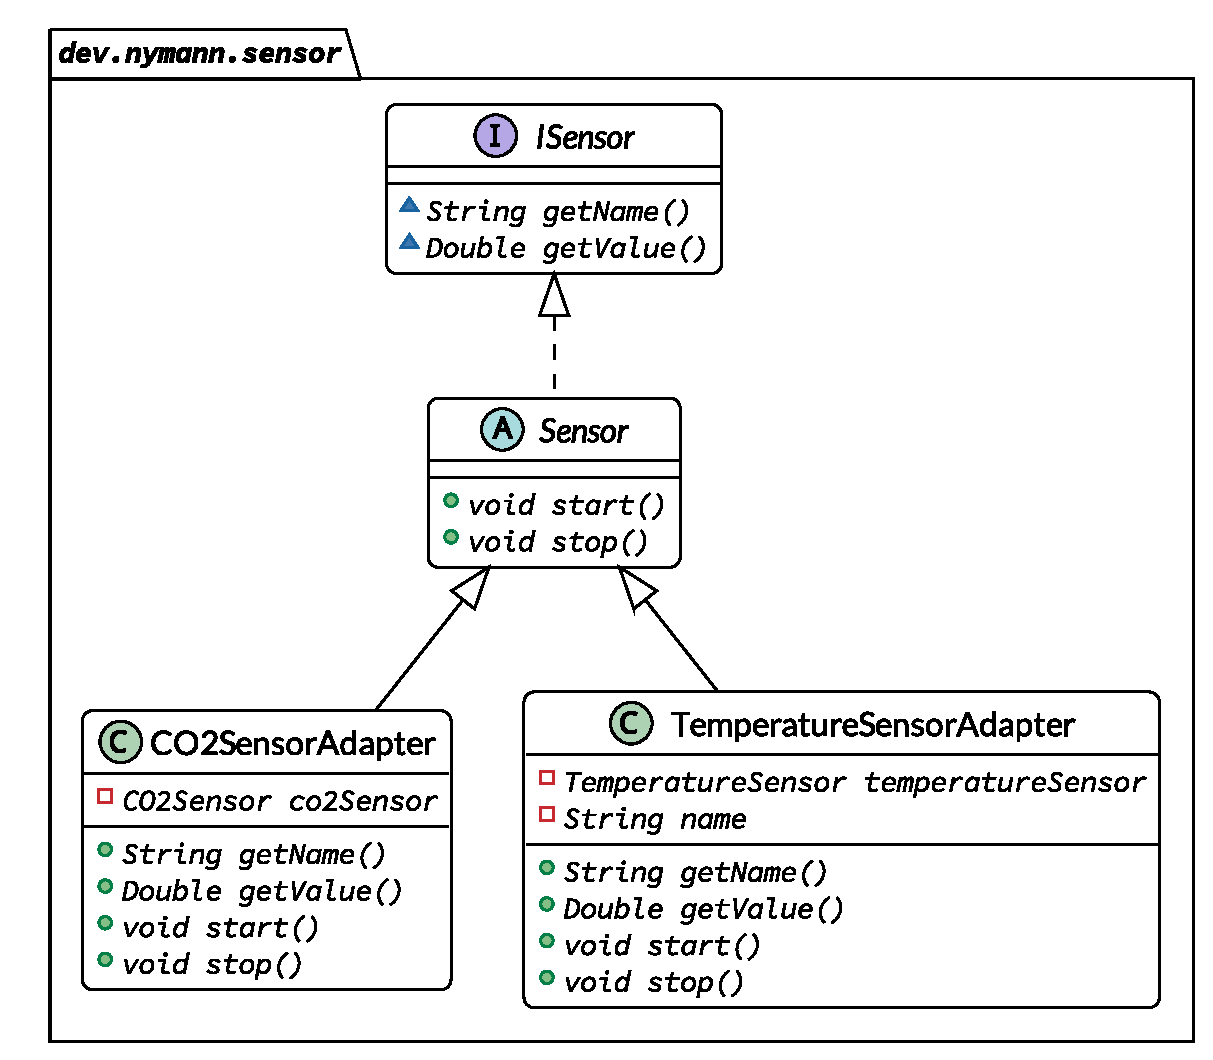
\includegraphics[scale=0.8]{part_two/sensor}
\end{figure}

\begin{figure}
\caption{CO2 Sensor}
\centering
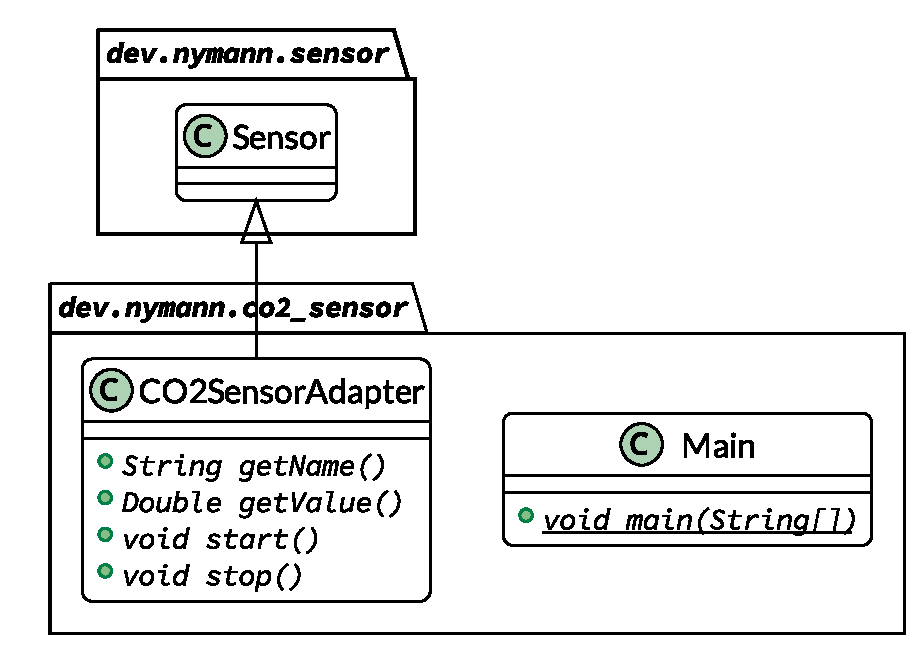
\includegraphics[scale=0.8]{part_two/co2-sensor}
\end{figure}

\begin{figure}
\caption{CO2 Sensor}
\centering
\includegraphics[scale=0.8]{part_two/temperature-sensor}
\end{figure}
